%% ------------------------------------------------------------------------- %%
\chapter{Ajuste dos hiper-parâmetros e normalização em lote}
\label{ape:ajuste-hiper-parametros-cnn}

Neste capítulo apresentamos os resultados dos ajustes dos hiper-parâmetros e da normalização em lote feita nas arquiteturas convolucional, \Gls{unif} e \textit{Embedding}. O intuito destes ajustes é obter um modelo mais robusto e evitar o \textit{overfitting}.

\section{Ajuste dos hiper-parâmetros da rede convolucional}
\label{sec:ajuste-hiper-parametros-cnn}

A rede convolucional exige alguns hiper-parâmetros que devem ser informados durante o treinamento. Estes hiper-parâmetros definem a capacidade do nosso modelo, o tipo de informação a ser extraída, a forma como as informações serão combinadas e o modo como as operações de convolução serão feitas. Os ajustes são importantes, pois auxiliam na obtenção de um modelo mais robusto, dado que alguns hiper-parâmetros controlam a capacidade do modelo, ou auxiliam na aprendizagem durante o treinamento, pois eles podem ajudar o modelo a correlacionar os dados, definindo o modo como as informações serão extraídas \citep{bengio-hyper-parameter-optimization-2012}. Para realizar estes ajustes, fizemos alguns experimentos alterando os hiper-parâmetros das redes convolucionais, juntamente com uma análise do comportamento dos modelos durante a aprendizagem. Além disso, verificamos o desempenho da redes convolucionais, com relação a métrica MRR, em uma amostra de pares de questões e trechos de códigos anotados manualmente, a fim de verificar se o modelo está conseguindo correlacionar os trechos de código-fonte relevantes às suas questões.

A rede convolucional exige três hiper-parâmetros: filtros, \textit{kernel} e \textit{stride}.
O parâmetro \textit{kernel} ou janela do filtro convolucional define o tamanho do quadro da operação de convolução. No nosso caso, que estamos utilizando a operação de convolução de 1 dimensão, Conv1D, o \textit{kernel} define os n-grams a serem extraídos do vetor de entrada. O ajuste neste parâmetro irá definir como a rede convolucional irá combinar as informações. Um \textit{kernel} de tamanho 2, indica que o modelo irá extrair bi-grams, enquanto um de tamanho 3, irá extrair um tri-gram e assim por diante. Em nosso caso, avaliamos o comportamento do modelo para tamanhos de \textit{kernel} 2, 3 e 4 e a junção de \textit{kernels} de tamanhos diferentes: 2, 3, 5 e 7. Segundo \cite{wen-joint-modeling-question-answer-2019}, a junção de filtros convolucionais com tamanhos de janelas diferentes levou a uma melhor aprendizagem e um melhor desempenho em uma tarefa de seleção de respostas.



Já o parâmetro filtros define a dimensão de saída da operação de convolução. Este parâmetro indica a quantidade de filtros no resultado da operação. E como cada filtro tenta extrair uma característica diferente do vetor de entrada, quanto maior a quantidade dos filtros, maior será a quantidade de características a serem extraídas pelo nosso modelo e maior será a sua capacidade. Para ajustar este parâmetro, analisamos a quantidade de filtros no intervalo de 1000 a 4000 conforme recomendação de \cite{feng-2015} e \cite{tan-lstm-qa}. Mas também avaliamos quantidades menores como 50, 100, 200 e 500. Os resultados podem ser visualizados na Seção~\ref{sec:ape-filtros}.


E o parâmetro \textit{stride} ou passo define a quantidade de posições que o filtro deslocar-se-á durante a operação de convolução. Optamos, em nosso caso, por manter o valor padrão 1 para o passo, i.e., o filtro deslocar-se-á por todas as posições do vetor de entrada de 1 (uma) em 1 (uma) posição.




\subsection{Filtros}
\label{sec:ape-filtros}

Para analisar como os filtros afetam o comportamento e desempenho das redes convolucionais, fixamos o parâmetro \textit{kernel} com o valor $2$, recomendação feita por \cite{tan-lstm-qa}, e executamos os testes com diferentes quantidades de filtros. Neste experimento, analisamos as seguintes quantidades: 50, 100, 200, 500, 1000, 2000, 4000. Conforme citado no capítulo~\ref{cap:experimento}, foram utilizadas $60.083$ amostras, sendo que $42058$ foram utilizadas para o conjunto de treinamento e $18025$ para o conjunto de validação. E a avaliação final foi feita conforme o procedimento descrito na Seção~\ref{sec:avaliacao}.



\begin{figure}[p]
\begin{subfigure}{.5\textwidth}
  \centering
  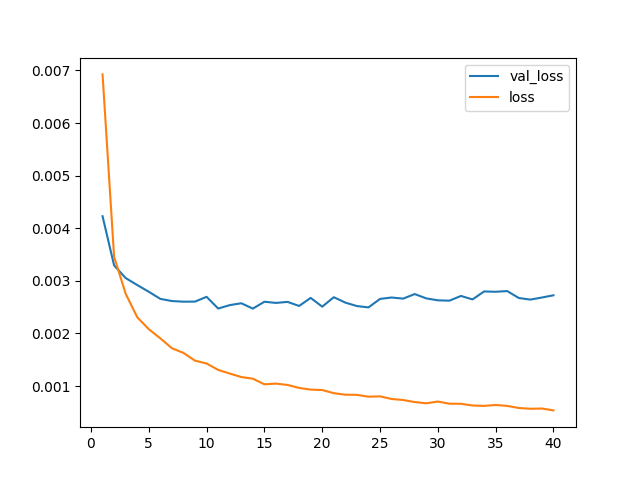
\includegraphics[width=.8\linewidth]{figuras/ape-ajustes-hiper-parametros/cnn-50-k-2.png}
  \caption{Rede convolucional com parâmetro $F = 50$}
  \label{fig:cnn-50-k-2}
\end{subfigure}%
\begin{subfigure}{.5\textwidth}
  \centering
  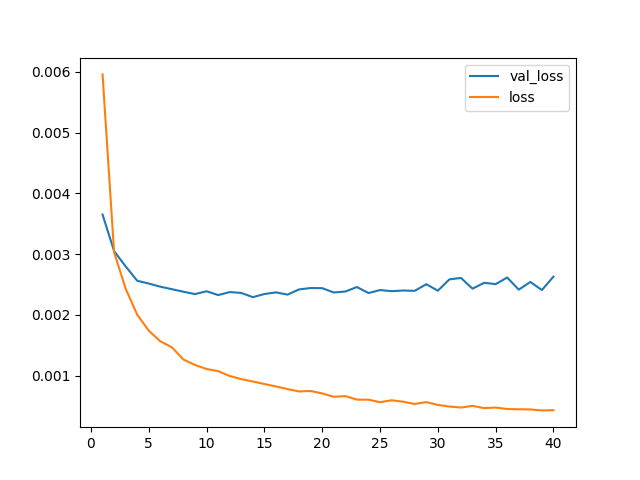
\includegraphics[width=.8\linewidth]{figuras/ape-ajustes-hiper-parametros/cnn-100-k-2.png}
  \caption{Rede convolucional com parâmetro $F = 100$}
  \label{fig:cnn-100-k-2}
\end{subfigure}
\begin{subfigure}{.5\textwidth}
  \centering
  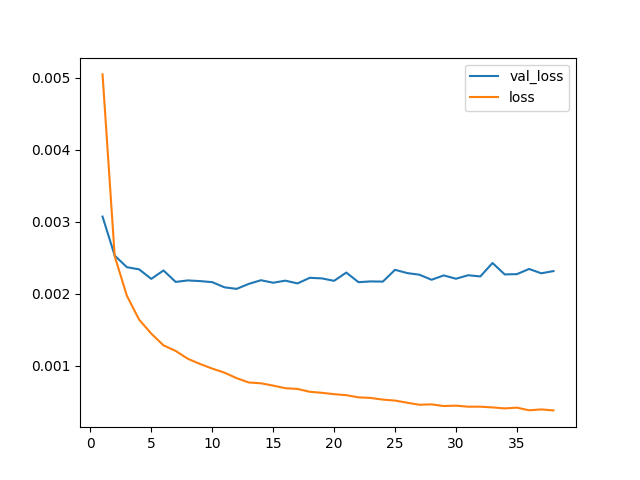
\includegraphics[width=.8\linewidth]{figuras/ape-ajustes-hiper-parametros/cnn-200-k-2.png}
  \caption{Rede convolucional com parâmetro $F = 200$}
  \label{fig:cnn-200-k-2}
\end{subfigure}
\begin{subfigure}{.5\textwidth}
  \centering
  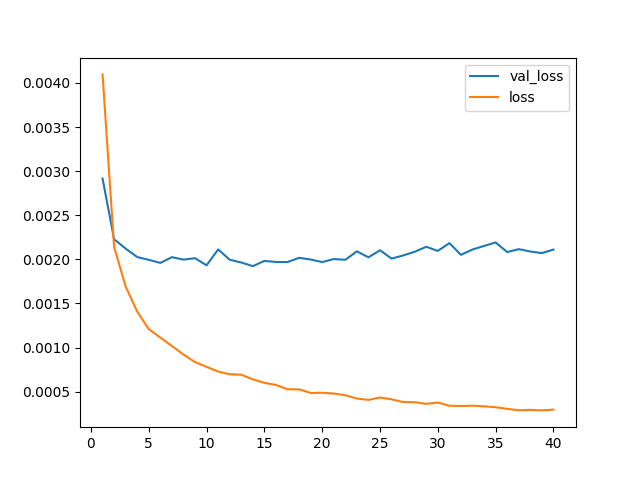
\includegraphics[width=.8\linewidth]{figuras/ape-ajustes-hiper-parametros/cnn-500-k-2.png}
  \caption{Rede convolucional com parâmetro $F = 500$}
  \label{fig:cnn-500-k-2}
\end{subfigure}
\begin{subfigure}{.5\textwidth}
  \centering
  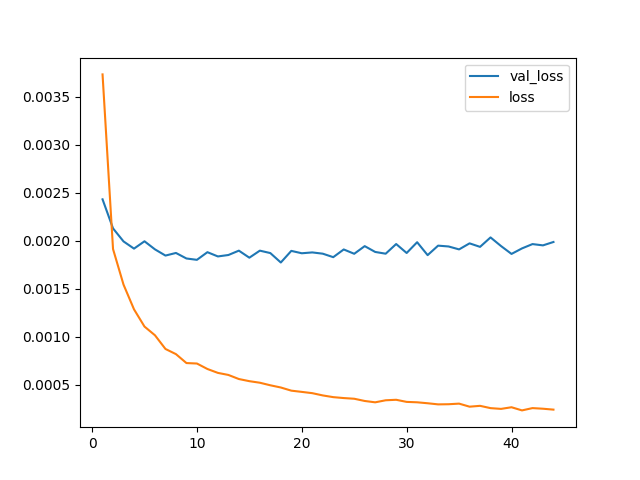
\includegraphics[width=.8\linewidth]{figuras/ape-ajustes-hiper-parametros/cnn-1000-k-2.png}
  \caption{Rede convolucional com parâmetro $F = 1000$}
  \label{fig:cnn-1000-k-2}
\end{subfigure}
\begin{subfigure}{.5\textwidth}
  \centering
  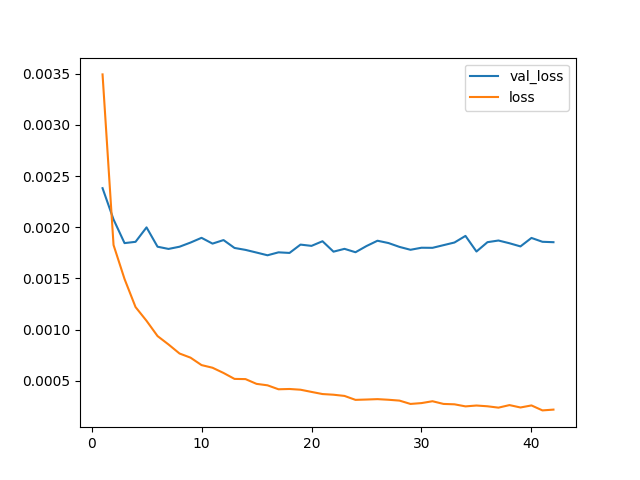
\includegraphics[width=.8\linewidth]{figuras/ape-ajustes-hiper-parametros/cnn-2000-k-2.png}
  \caption{Rede convolucional com parâmetro $F = 2000$}
  \label{fig:cnn-2000-k-2}
\end{subfigure}
\begin{subfigure}{.5\textwidth}
  \centering
  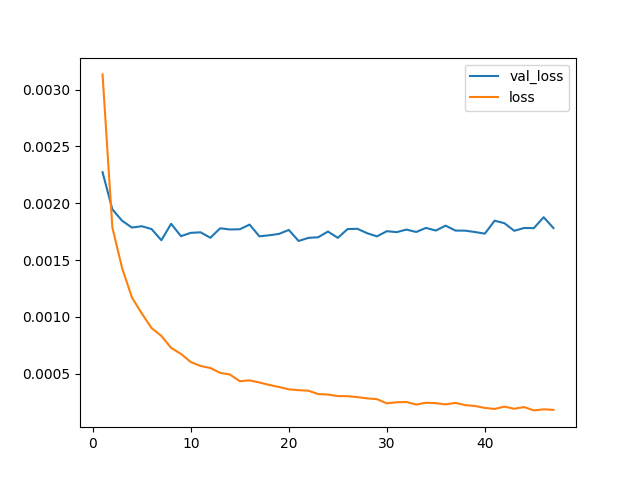
\includegraphics[width=.8\linewidth]{figuras/ape-ajustes-hiper-parametros/cnn-4000-k-2.png}
  \caption{Rede convolucional com parâmetro $F = 4000$}
  \label{fig:cnn-4000-k-2}
\end{subfigure}
\caption{Este gráfico apresenta um comparativo do erro no conjunto de validação em comparação com o erro no conjunto de treinamento. Mais detalhes sobre o treinamento, ver a Seção~\ref{sec:treinamento}. Arquitetura de rede convolucional proposta no Capítulo~\ref{cap:abordagem}, ver Figura~\ref{fig:cnn-architecture}. Hiper-parâmetros: $m = 0.009$, $k = 2$. O parâmetro F indica a quantidade de filtros convolucionais. Nas figuras de \emph{a} a \emph{g}, o eixo \emph{y} indica o valor de erro da função de perda \textit{hinge}, já o eixo \emph{x} indica as épocas de treinamento. A legenda \emph{val\_loss} das figuras de \emph{a} a \emph{g} indica o erro na amostra de validação e a legenda \emph{loss} indica o valor do erro na amostra de treinamento. }
\label{fig:treinamento-cnn-k-2-m-0009}
\end{figure}


\begin{table}[H]
\centering
\begin{tabular}{ p{1cm} p{4cm} P{4cm} }
 \hline
   & Modelos & \textbf{Resultados MRR}\\
 \hline

 C1 & CNN / F = 50 &  $0.564$\\
 
 C2 & CNN / F = 100 &  $0.587$\\
 
 C3 & CNN / F = 200 &  $0.624$\\
 
 C4 & CNN / F = 500 &  $0.639$\\
 
 C5 & CNN / F = 1000 &  $0.654$\\
 
 C6 & CNN / F = 2000 &  $0.675$\\
 
 C7 & CNN / F = 4000 &  $0.664$\\
 
\hline
\end{tabular}
\caption{Resultado da avaliação dos modelos CNN na amostra EVAL. MRR refere-se a média do resultado do Mean Reciprocal Rank (equação~\ref{eq:mrr}). F indica a quantidade de filtros convolucionais utilizados durante o treinamento das redes convolucionais. Os hiper-parâmetros utilizados foram: $K = 2$ e  $m = 0,009$.}
\label{table:cnn-filtros}
\end{table}

De acordo com a Figura~\ref{fig:treinamento-cnn-k-2-m-0009}, o aumento da quantidade de filtros diminuiu o valor do erro na amostra de validação. O valor de erro que era em torno de $0,003$ na Figura~\ref{fig:cnn-50-k-2}, diminuiu pela metade, ficando em torno de $0.0015$ nas Figuras~\ref{fig:cnn-2000-k-2} e \ref{fig:cnn-4000-k-2}, para a quantidade de filtros entre 2000 e 4000. Este aumento influenciou também o desempenho, conforme os resultados apontados na Tabela~\ref{table:cnn-filtros}. Houve um aumento de aproximadamente 20\% quando comparamos o pior resultado com o melhor resultado (linhas C1 e C6). Porém, podemos observar que o comportamento do modelo começa a dar sinais de \textit{overfitting}, onde o valor do erro na amostra de treinamento cai abruptamente, enquanto o erro na amostra de validação permance estável e começa a aumentar. Para lidar com este problema, optamos por utilizar a normalização em lote e verificar a sua eficácia na regularização do nosso modelo. Os resultados da normalização em lote podem ser visualizadas na Seção~\ref{sec:regularizacao-normalizacao-lote}. 

\subsection{\textit{Kernel}}

Conforme exibido no Capítulo~\ref{cap:abordagem}, o \textit{kernel} define na rede convolucional de 1 dimensão, Conv1D, o modo como as características do vetor de entrada serão combinadas. Caso o \textit{kernel} tenha tamanho 2, o filtro convolucional irá extrair as características latentes através da combinação em bi-grams, por exemplo. Para avaliar como esta combinação afeta o desempenho do modelo, analisamos diferentes valores para o \textit{kernel}. Fixamos o parâmetro margem da função de perda \textit{hinge} em $0,009$ e comparamos apenas os modelos com a quantidade de filtros 1000, 2000 e 4000. 

\begin{table}[H]
\centering
\begin{tabular}{ p{1cm} p{3cm} P{2.2cm} P{2.2cm} P{2.2cm} P{2.8cm} }
 \hline
    & & \multicolumn{4}{c}{\textbf{Resultados MRR}}\\
 \hline
 & \textbf{Modelos} & \textbf{$K = 2$} & \textbf{$K = 3$} & \textbf{$K = 4$}& \textbf{$K = [2, 3, 5, 7]$}\\
 \hline

 C1 & CNN / F = 1000 & $0.654 $ & $0.660$& $0.652$& $0.676$\\
 
 C2 & CNN / F = 2000 & $0.675 $ & $0.683$& $0.662$& $0.683$\\
 
 C3 & CNN / F = 4000 & $0.664$ & $0.674$& $0.680$& $0.677$\\
 
\hline
\end{tabular}
\caption{Resultado da avaliação dos modelos CNN na amostra EVAL. MRR refere-se a média do resultado do Mean Reciprocal Rank (equação~\ref{eq:mrr}). F indica a quantidade de filtros convolucionais utilizados durante o treinamento das redes convolucionais. Utilizamos o parâmetro $m = 0,009$ para a função de perda \textit{hinge}.}
\label{table:cnn-kernel}
\end{table}


\begin{figure}[H]
\begin{subfigure}{.5\textwidth}
  \centering
  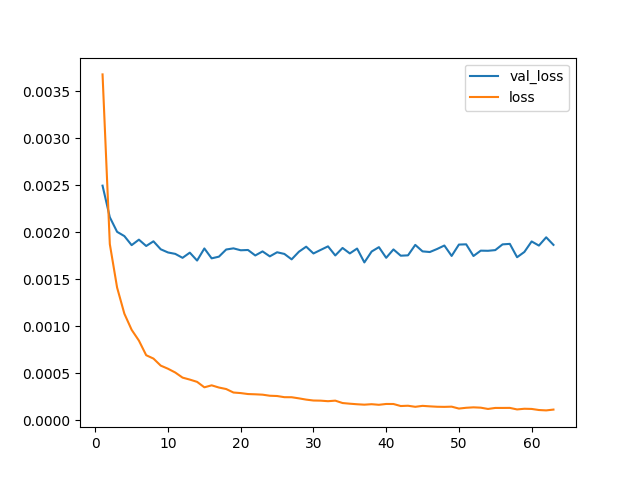
\includegraphics[width=.8\linewidth]{figuras/ape-ajustes-hiper-parametros/cnn-1000.png}
  \caption{Rede convolucional com parâmetros $F = 1000$ e $K = [2,3,5,7]$}
  \label{fig:cnn-1000}
\end{subfigure}%
\begin{subfigure}{.5\textwidth}
  \centering
  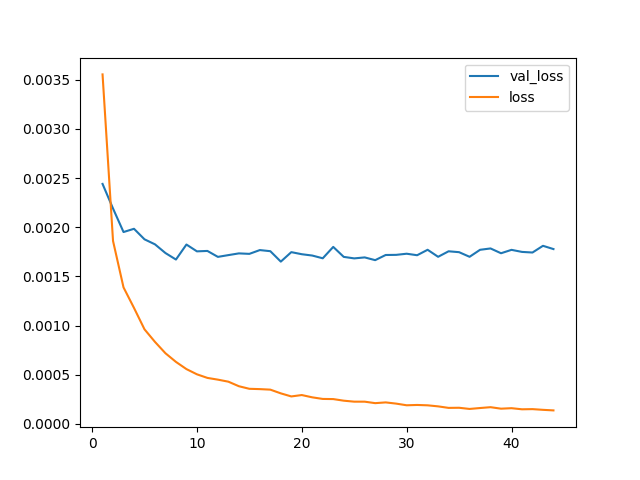
\includegraphics[width=.8\linewidth]{figuras/ape-ajustes-hiper-parametros/cnn-2000.png}
  \caption{Rede convolucional com parâmetros $F = 2000$ e $K = [2, 3, 5, 7]$}
  \label{fig:cnn-2000}
\end{subfigure}
\begin{subfigure}{.5\textwidth}
  \centering
  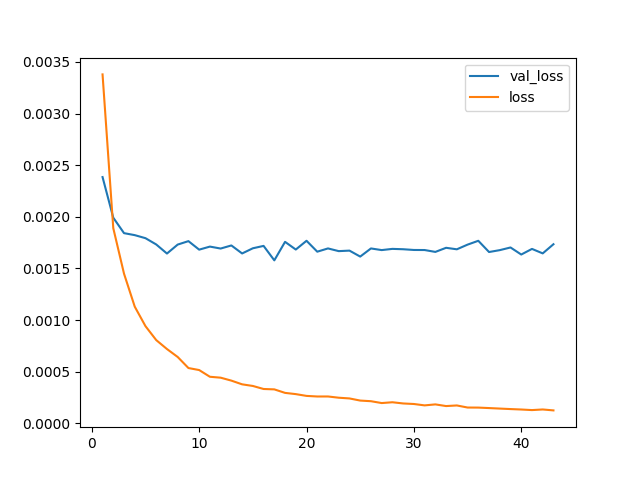
\includegraphics[width=.8\linewidth]{figuras/ape-ajustes-hiper-parametros/cnn-4000.png}
  \caption{Rede convolucional com parâmetros $F = 4000$ e $K = [2, 3, 5, 7]$}
  \label{fig:cnn-4000}
\end{subfigure}
\begin{subfigure}{.5\textwidth}
  \centering
  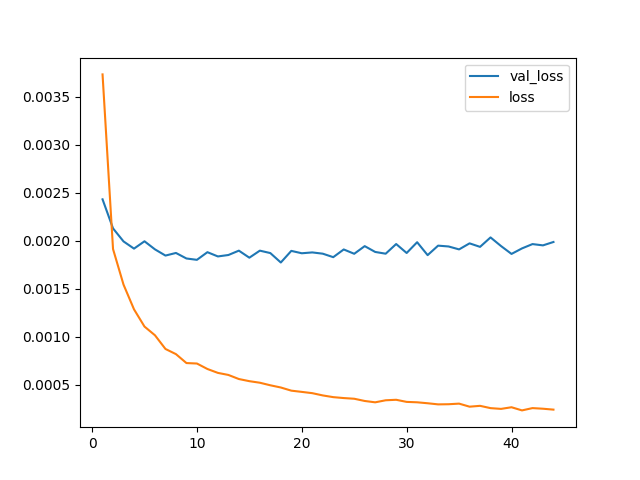
\includegraphics[width=.8\linewidth]{figuras/ape-ajustes-hiper-parametros/cnn-1000-k-2.png}
  \caption{Rede convolucional com parâmetros $F = 1000$ e $K = 2$}
  \label{fig:cnn-1000-k-2-v2}
\end{subfigure}
\begin{subfigure}{.5\textwidth}
  \centering
  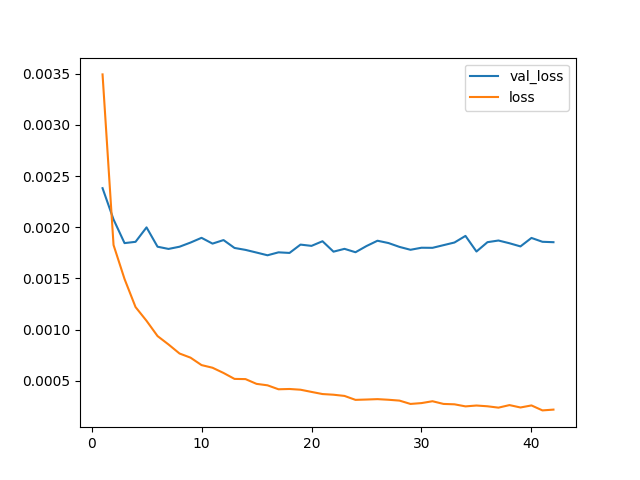
\includegraphics[width=.8\linewidth]{figuras/ape-ajustes-hiper-parametros/cnn-2000-k-2.png}
  \caption{Rede convolucional com parâmetros $F = 2000$ e $K = 2$}
  \label{fig:cnn-2000-k-2-v2}
\end{subfigure}
\begin{subfigure}{.5\textwidth}
  \centering
  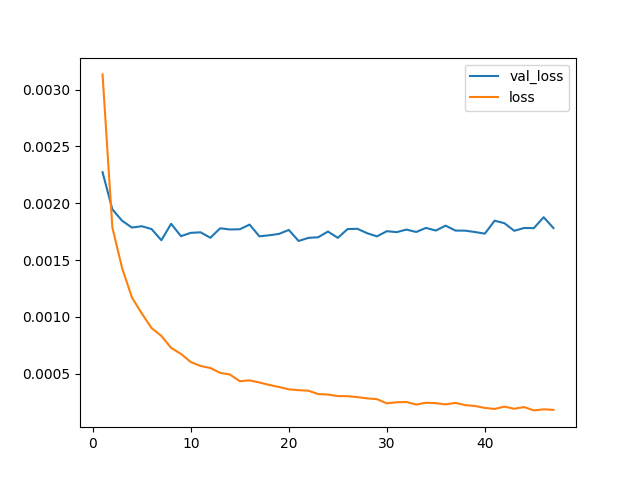
\includegraphics[width=.8\linewidth]{figuras/ape-ajustes-hiper-parametros/cnn-4000-k-2.png}
  \caption{Rede convolucional com parâmetros $F = 4000$ e $K = 2$}
  \label{fig:cnn-4000-k-2-v2}
\end{subfigure}
\caption{Gráfico do treinamento da rede convolucional na recuperação de trecho de código-fonte. Este gráfico apresenta um comparativo do erro no conjunto de validação em comparação com o erro no conjunto de treinamento. Mais detalhes sobre o treinamento, ver a Seção~\ref{sec:treinamento}. Arquitetura de rede convolucional proposta no Capítulo~\ref{cap:abordagem}, ver Figura~\ref{fig:cnn-architecture}. Hiper-parâmetros: $m = 0.009$. O parâmetro F indica a quantidade de filtros convolucionais, o parâmetro K indica o tamanho da janela do filtro convolucional. Nas figuras de \emph{a} a \emph{f}, o eixo \emph{y} indica o valor de erro da função de perda \textit{hinge}, já o eixo \emph{x} indica as épocas de treinamento. A legenda \emph{val\_loss} das figuras de \emph{a} a \emph{g} indica o erro na amostra de validação e a legenda \emph{loss} indica o valor do erro na amostra de treinamento. }
\label{fig:treinamento-cnn-diferentes-kernels}
\end{figure}

\begin{figure}[H]
\begin{subfigure}{.5\textwidth}
  \centering
  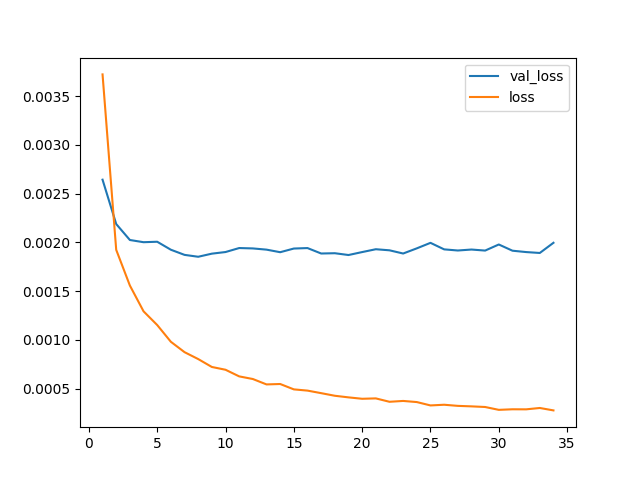
\includegraphics[width=.8\linewidth]{figuras/ape-ajustes-hiper-parametros/cnn-1000-k-3.png}
  \caption{Rede convolucional com parâmetros $F = 1000$ e $K = 3$}
  \label{fig:cnn-1000-k-3}
\end{subfigure}
\begin{subfigure}{.5\textwidth}
  \centering
  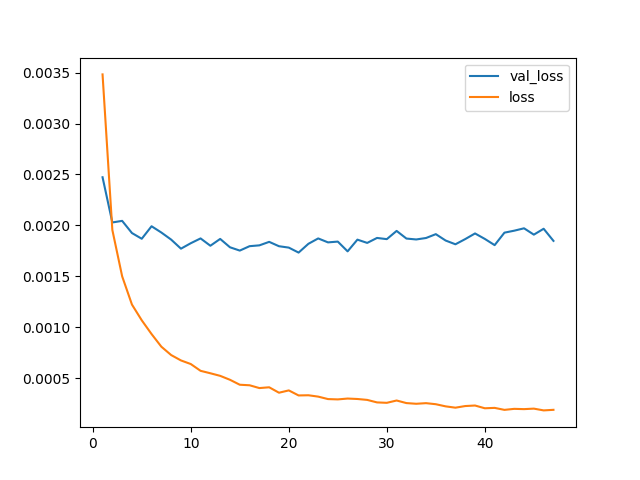
\includegraphics[width=.8\linewidth]{figuras/ape-ajustes-hiper-parametros/cnn-2000-k-3.png}
  \caption{Rede convolucional com parâmetros $F = 2000$ e $K = 3$}
  \label{fig:cnn-2000-k-3}
\end{subfigure}
\begin{subfigure}{.5\textwidth}
  \centering
  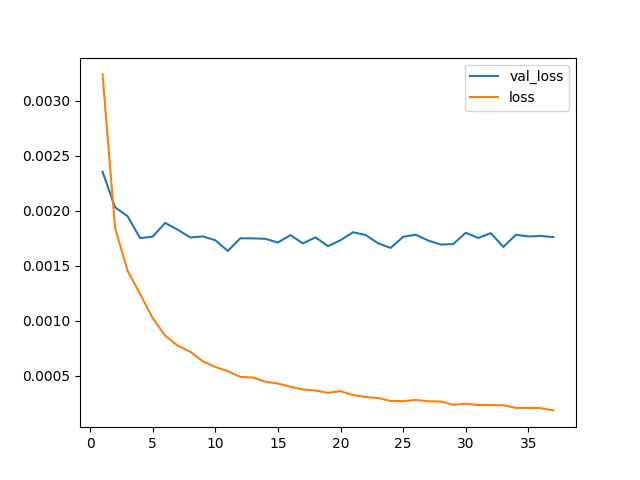
\includegraphics[width=.8\linewidth]{figuras/ape-ajustes-hiper-parametros/cnn-4000-k-3.png}
  \caption{Rede convolucional com parâmetros $F = 4000$ e $K = 3$}
  \label{fig:cnn-4000-k-3}
\end{subfigure}
\begin{subfigure}{.5\textwidth}
  \centering
  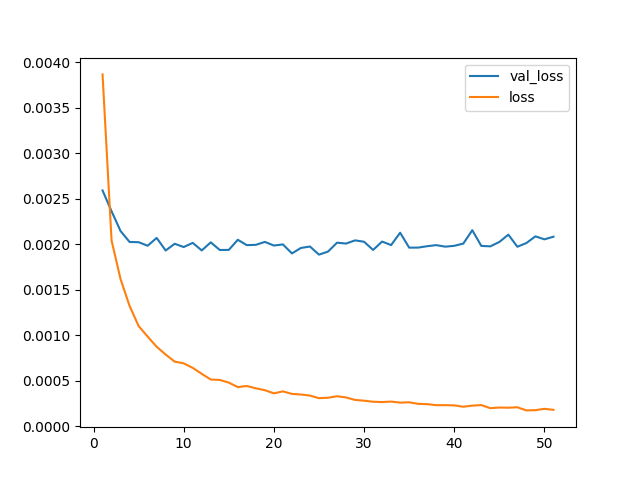
\includegraphics[width=.8\linewidth]{figuras/ape-ajustes-hiper-parametros/cnn-1000-k-4.png}
  \caption{Rede convolucional com parâmetros $F = 1000$ e $K = 4$}
  \label{fig:cnn-1000-k-4}
\end{subfigure}
\begin{subfigure}{.5\textwidth}
  \centering
  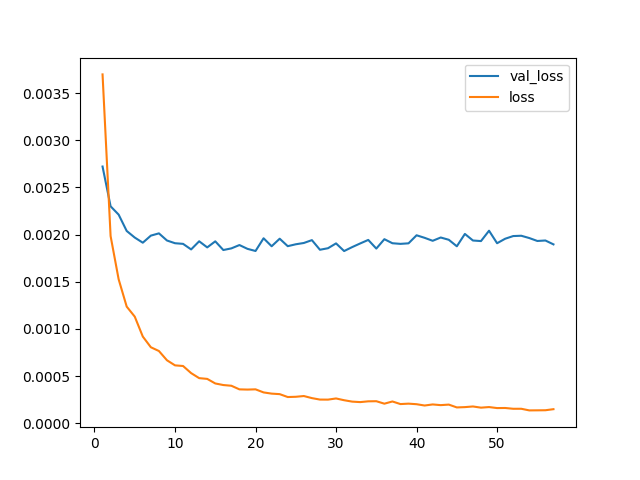
\includegraphics[width=.8\linewidth]{figuras/ape-ajustes-hiper-parametros/cnn-2000-k-4.png}
  \caption{Rede convolucional com parâmetros $F = 2000$ e $K = 4$}
  \label{fig:cnn-2000-k-4}
\end{subfigure}
\begin{subfigure}{.5\textwidth}
  \centering
  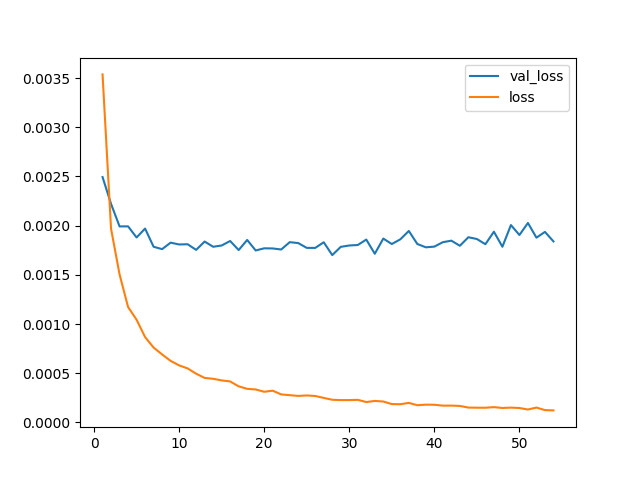
\includegraphics[width=.8\linewidth]{figuras/ape-ajustes-hiper-parametros/cnn-4000-k-4.png}
  \caption{Rede convolucional com parâmetros $F = 4000$ e $K = 4$}
  \label{fig:cnn-4000-k-4}
\end{subfigure}
\caption{Gráfico do treinamento da rede convolucional na recuperação de trecho de código-fonte. Este gráfico apresenta um comparativo do erro no conjunto de validação em comparação com o erro no conjunto de treinamento. Mais detalhes sobre o treinamento, ver a Seção~\ref{sec:treinamento}. Arquitetura de rede convolucional proposta no Capítulo~\ref{cap:abordagem}, ver Figura~\ref{fig:cnn-architecture}. Hiper-parâmetros: $m = 0.009$. O parâmetro F indica a quantidade de filtros convolucionais, o parâmetro K indica o tamanho da janela do filtro convolucional. Nas figuras de \emph{a} a \emph{f}, o eixo \emph{y} indica o valor de erro da função de perda \textit{hinge}, já o eixo \emph{x} indica as épocas de treinamento. A legenda \emph{val\_loss} das figuras de \emph{a} a \emph{g} indica o erro na amostra de validação e a legenda \emph{loss} indica o valor do erro na amostra de treinamento. }
\label{fig:treinamento-cnn-diferentes-kernels-2}
\end{figure}


Verificamos o comportamento para os tamanhos 2, 3, 4 e a combinação de tamanhos 2, 3, 5 e 7. Conforme as Figuras~\ref{fig:treinamento-cnn-diferentes-kernels} e \ref{fig:treinamento-cnn-diferentes-kernels-2}, não houve melhora significativa na diferença entre o erro de validação e o erro de treinamento para kernels de tamanho 3 e 4 em comparação com o kernel de tamanho 2. A diferença entre o erro de validação e erro de treinamento é um indicativo para sabermos se o modelo está conseguindo aprender ou se temos um problema de \textit{overfitting} ou \textit{underfitting}. Em nosso caso, podemos ver pelas Figuras~\ref{fig:treinamento-cnn-diferentes-kernels} e \ref{fig:treinamento-cnn-diferentes-kernels-2}, que o nosso modelo está com problema de \textit{overfitting}, onde há uma grande diferença entre o erro de validação e erro de treinamento. Para sabermos qual \textit{kernel} escolher, verificamos também o desempenho dos modelos na amostra EVAL (mais detalhes sobre esta amostra na Seção~\ref{sec:conjunto-dados-avaliacao-treinamento}). Conforme os resultados apontados na Tabela~\ref{table:cnn-kernel}, não houve uma melhora significativa entre o \textit{kernel} de tamanho 2 e o restante dos \textit{kernels}. Neste caso, optamos por manter o kernel fixado em $2$, conforme \cite{tan-lstm-qa} haviam recomendado.


\subsection{Regularização - Normalização em Lote}
\label{sec:regularizacao-normalizacao-lote}

Conforme as Figuras~\ref{fig:cnn-1000-k-2-v2}, \ref{fig:cnn-2000-k-2-v2} e \ref{fig:cnn-4000-k-2-v2}, as redes convolucionais estão dando sinais de \textit{overfitting}, onde o valor do erro na amostra de treinamento está diminuindo rapidamente, enquanto o valor do erro na amostra de validação está estável e aumentando ao longo do tempo. Para tentar redimir este problema, aplicamos a normalização em lote para regularizar o nosso modelo. Conforme \cite{sergey-batch-normalization-2015}, a aprendizagem em redes neurais profundas é complicada, pois a distribuição de cada camada é alterada, conforme os parâmetros são atualizados ao longo do treinamento. Isto requer uma otimização e ajuste dos parâmetros a fim de evitar a saturação das funções de ativação. Para mitigar este problema e auxiliar o modelo a aprender de maneira mais rápida, os pesquisadores apresentaram a normalização em lote, que permite utilizarmos taxas de aprendizagem mais altas e não requer muitos cuidados na inicialização do modelo. Além disso, segundo os próprios pesquisadores, a normalização em lote auxilia numa aprendizagem mais rápida, diminuindo o número de épocas de treinamento, além de ajudar na melhora do desempenho e na obtenção de um modelo mais robusto, não necessitando de outras técnicas de regularização como \textit{dropout} \citep{sergey-batch-normalization-2015}.

Aplicamos a normalização em lote nas redes convolucionais e podemos notar uma sutil melhora na aprendizagem de acordo com as Figuras~\ref{fig:treinamento-cnn-normalizacao-em-lote}. Houve uma melhora principalmente para as primeiras 25 épocas iniciais, onde há uma leve diminuição entre o valor do erro na amostra de treinamento em comparação com o erro na amostra de validação. Esta sutil melhora ocorre principalmente para os modelos com uma quantidade maior de filtros. Em nosso caso, quando os valores estão entre 2000 e 4000.

Podemos notar também que a normalização em lote auxiliou as redes convolucionais com 1000 e 2000 filtros a tornaram-se mais estáveis (Figuras~\ref{fig:cnn-1000-k-2-m-005-normalizacao-em-lote} e \ref{fig:cnn-2000-k-2-m-005-normalizacao-em-lote}), mas isto não ocorreu para a rede convolucional com 4000 filtros (Figura~\ref{fig:cnn-4000-k-2-m-005-normalizacao-em-lote}). Ao analisarmos o comportamento da rede convolucional com 4000 filtros, percebemos que aprendizagem ocorreu de forma mais estável para as 15 primeiras épocas iniciais. Porém, na época 25 ocorre um ''grande salto'' e temos uma enorme diferença entre o erro de validação e o erro de treinamento. Para mitigar este problema, adotamos a parada antecipada do treinamento. Conforme explicado na Seção~\ref{sec:treinamento}, caso não haja diminuição do valor do erro na amostra de validação durante 25 épocas consecutivas, o treinamento é interrompido e o modelo que obtiver a maior média MRR na amostra DEV (mais detalhes sobre esta amostra na Seção~\ref{sec:conjunto-dados}) é escolhido.

\begin{figure}[H]
\begin{subfigure}{.5\textwidth}
  \centering
  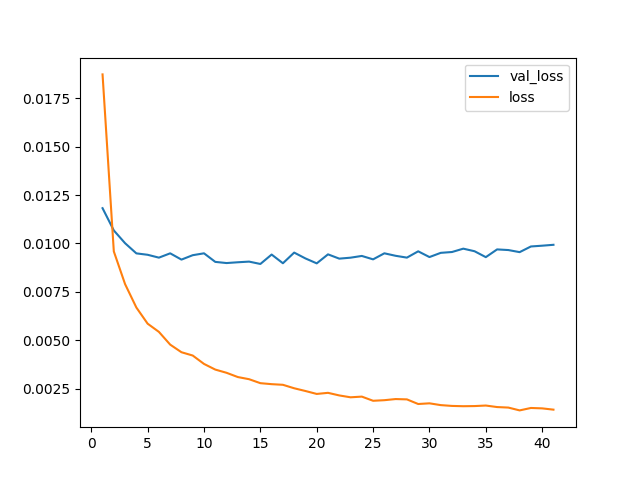
\includegraphics[width=.8\linewidth]{figuras/ape-ajustes-hiper-parametros/cnn-1000-k-2-m-005.png}
  \caption{Rede convolucional com parâmetros $F = 1000$, $K = 2$ e $m = 0,05$.}
  \label{fig:cnn-1000-k-2-m-005}
\end{subfigure}
\begin{subfigure}{.5\textwidth}
  \centering
  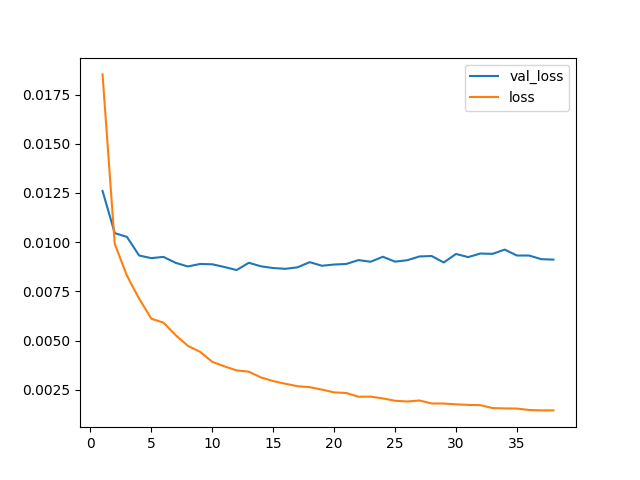
\includegraphics[width=.8\linewidth]{figuras/ape-ajustes-hiper-parametros/cnn-with-bn-1000-k-2-m-005.png}
  \caption{Rede convolucional com parâmetros $F = 1000$, $K = 2$ e $m = 0,05$ e normalização em lote.}
  \label{fig:cnn-1000-k-2-m-005-normalizacao-em-lote}
\end{subfigure}
\begin{subfigure}{.5\textwidth}
  \centering
  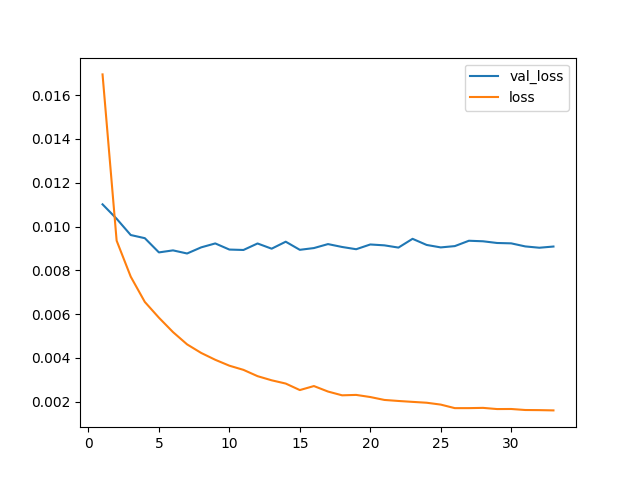
\includegraphics[width=.8\linewidth]{figuras/ape-ajustes-hiper-parametros/cnn-2000-k-2-m-005.png}
  \caption{Rede convolucional com parâmetros $F = 2000$, $K = 2$ e $m = 0,05$.}
  \label{fig:cnn-2000-k-2-m-005}
\end{subfigure}
\begin{subfigure}{.5\textwidth}
  \centering
  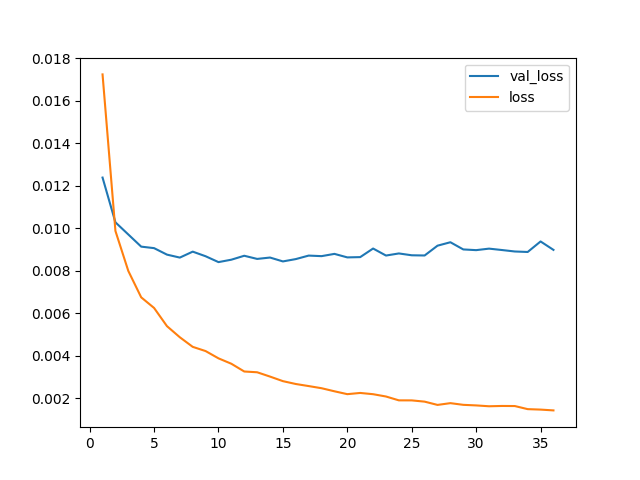
\includegraphics[width=.8\linewidth]{figuras/ape-ajustes-hiper-parametros/cnn-with-bn-2000-k-2-m-005.png}
  \caption{Rede convolucional com parâmetros $F = 2000$, $K = 2$ e $m = 0,05$ e normalização em lote.}
  \label{fig:cnn-2000-k-2-m-005-normalizacao-em-lote}
\end{subfigure}
\begin{subfigure}{.5\textwidth}
  \centering
  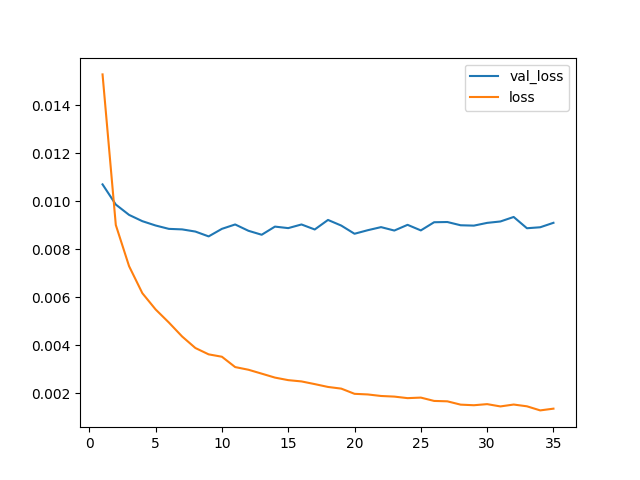
\includegraphics[width=.8\linewidth]{figuras/ape-ajustes-hiper-parametros/cnn-4000-k-2-m-005.png}
  \caption{Rede convolucional com parâmetros $F = 4000$, $K = 2$ e $m = 0,05$.}
  \label{fig:cnn-4000-k-2-m-005}
\end{subfigure}
\begin{subfigure}{.5\textwidth}
  \centering
  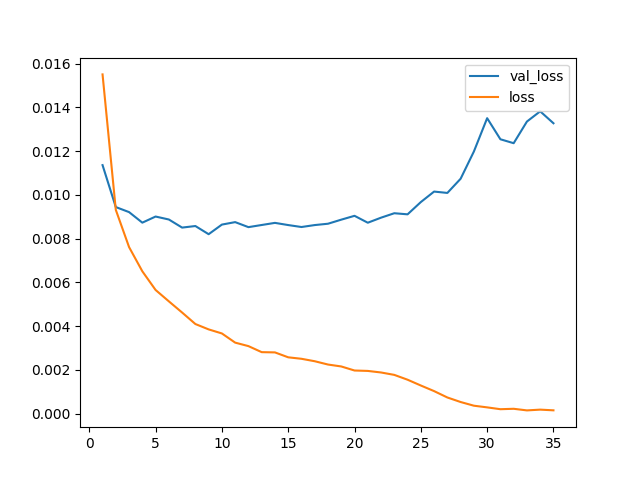
\includegraphics[width=.8\linewidth]{figuras/ape-ajustes-hiper-parametros/cnn-with-bn-4000-k-2-m-005.png}
  \caption{Rede convolucional com parâmetros $F = 4000$, $K = 2$ e $m = 0,05$ e normalização em lote.}
  \label{fig:cnn-4000-k-2-m-005-normalizacao-em-lote}
\end{subfigure}

\caption{Gráfico do treinamento da rede convolucional na recuperação de trecho de código-fonte. Este gráfico apresenta um comparativo do erro no conjunto de validação em comparação com o erro no conjunto de treinamento. Mais detalhes sobre o treinamento, ver a Seção~\ref{sec:treinamento}. O parâmetro F indica a quantidade de filtros convolucionais, o parâmetro K indica o tamanho da janela do filtro convolucional e o parâmetro \emph{m} é a margem utilizada na função de perda \textit{hinge}. Nas figuras de \emph{a} a \emph{f}, o eixo \emph{y} indica o valor de erro da função de perda \textit{hinge}, já o eixo \emph{x} indica as épocas de treinamento. A legenda \emph{val\_loss} das figuras de \emph{a} a \emph{g} indica o erro na amostra de validação e a legenda \emph{loss} indica o valor do erro na amostra de treinamento. Nas figuras do lado esquerdo: \emph{a}, \emph{c} e \emph{e} apresentam o comportamento das redes convolucionais durante o treinamento sem utilização de regularização. As figuras do lado direito: \emph{b}, \emph{d} e \emph{f} apresentam o comportamento das redes convolucionais utilizando normalização em lote. }
\label{fig:treinamento-cnn-normalizacao-em-lote}
\end{figure}

Apesar do ''grande salto'' para a rede convolucional com 4000 filtros, a normalização em lote melhorou o desempenho em todas as redes convolucionais. Conforme a Tabela~\ref{table:tabela-normalizacao-em-lote-cnn}, podemos verificar que houve um aumento do valor do MRR na amostra EVAL. Para nós, isto é um indicativo de que a normalização em lote auxiliou na aprendizagem. Além disso, a parada antecipada impediu o \textit{overfitting} do modelo, permitindo que selecionássemos o melhor candidato à avaliação final na amostra EVAL. Para termos um comparativo dos resultados nos testes finais, optamos por apresentar os valores finais do MRR de ambos os modelos, as redes convolucionais com normalização em lote e as redes sem normalização, na Seção~\ref{sec:resultados-avaliacao}.

\begin{table}[H]
\centering
\begin{tabular}{ p{1cm} p{4cm} P{4cm} P{4cm} }
 \hline
    & & \multicolumn{2}{c}{\textbf{Resultados MRR}}\\
 \hline
 & \textbf{Modelos} & \textbf{Sem NL} & \textbf{Com NL}\\
 \hline
 
 C1 & CNN / F = 1000 &  $0.669$&  \cellcolor{Gray!35}$0.682$\\
 
 C2 & CNN / F = 2000 &  $0.673$&  \cellcolor{Gray!35}$0.689$\\
 
 C3 & CNN / F = 4000 &  $0.687$& \cellcolor{Gray!35} $0.688$\\
 
\hline
\end{tabular}
\caption{Resultado da avaliação dos modelos CNN na amostra EVAL. MRR refere-se a média do resultado do Mean Reciprocal Rank (equação~\ref{eq:mrr}). F indica a quantidade de filtros convolucionais utilizados durante o treinamento das redes convolucionais. \emph{NL} é o acrônimo de Normalização em Lote. As células destacadas indicam qual o modelo obteve o melhor desempenho durante a avaliação. Os hiper-parâmetros utilizados foram: $K = 2$ e  $m = 0,05$.}
\label{table:tabela-normalizacao-em-lote-cnn}
\end{table}

\subsection{Compartilhamento de parâmetros}

Em nossos experimentos, comparamos o desempenho das redes convolucionais que compartilham os parâmetros entre as camadas das questões e trechos de código-fonte com as redes convolucionais que aprendem as representações de forma independente. Conforme as Figuras~\ref{fig:treinamento-shared-cnn}, podemos perceber que não houve uma alteração significativa no comportamento dos modelos durante a aprendizagem. Porém, ao analisarmos o desempenho com relação a métrica MRR, verificamos que houve uma melhora. Esta melhora de desempenho foi notada também por \cite{wen-joint-modeling-question-answer-2019}, onde eles apontaram que as redes convolucionais que aprendem as representações de forma independente, exploram de forma ineficiente a correlação semântica entre os pares de questões e respostas. E segundo os resultados apontados na Tabela~\ref{table:tabela-shared-cnn} e também na Seção~\ref{sec:resultados-avaliacao}, os modelos que compartilharam os parâmetros tiveram um desempenho, em média, 3\% superior. Para termos um comparativo, exibimos na Seção~\ref{sec:resultados-avaliacao} os resultados dos modelos que compartilham os parâmetros e também os resultados dos modelos que aprendem as representações de forma indepedente.

\begin{figure}[H]
\begin{subfigure}{.5\textwidth}
  \centering
  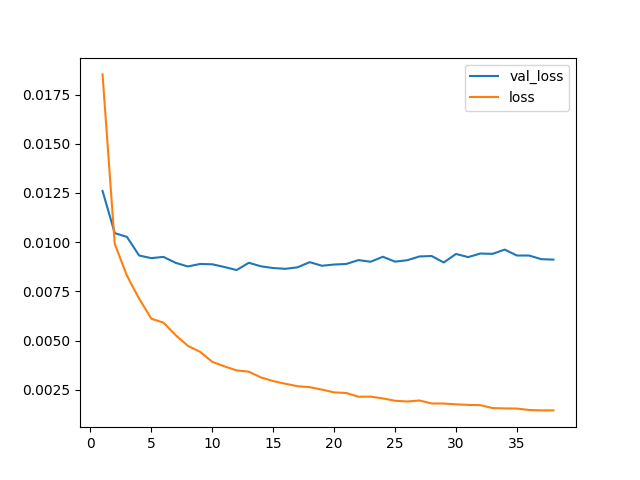
\includegraphics[width=.8\linewidth]{figuras/ape-ajustes-hiper-parametros/cnn-with-bn-1000-k-2-m-005.png}
  \caption{Rede convolucional com parâmetros $F = 1000$, $K = 2$ e $m = 0,05$ e normalização em lote.}
  \label{fig:cnn-1000-k-2-m-005-normalizacao-em-lote-v2}
\end{subfigure}
\begin{subfigure}{.5\textwidth}
  \centering
  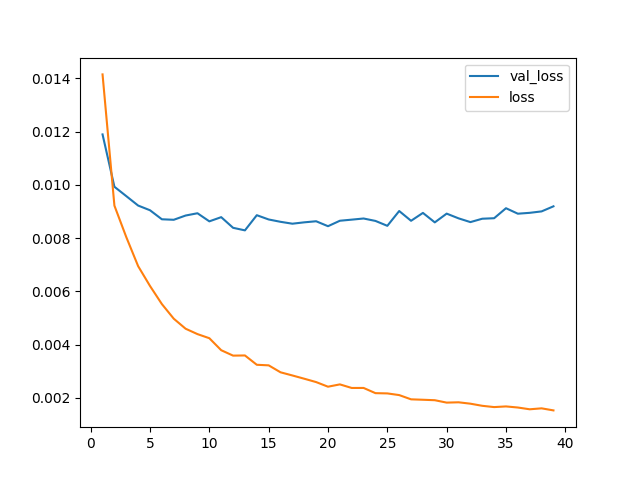
\includegraphics[width=.8\linewidth]{figuras/ape-ajustes-hiper-parametros/shared-cnn-with-bn-1000-k-2-m-005.png}
  \caption{Rede convolucional com parâmetros $F = 1000$, $K = 2$ e $m = 0,05$, normalização em lote e parâmetros compartilhado.}
  \label{fig:shared-cnn-1000-k-2-m-005-normalizacao-em-lote}
\end{subfigure}
\begin{subfigure}{.5\textwidth}
  \centering
  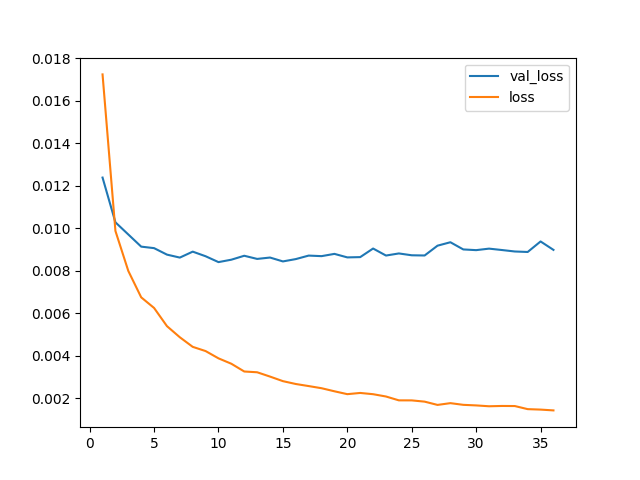
\includegraphics[width=.8\linewidth]{figuras/ape-ajustes-hiper-parametros/cnn-with-bn-2000-k-2-m-005.png}
  \caption{Rede convolucional com parâmetros $F = 2000$, $K = 2$ e $m = 0,05$ e normalização em lote.}
  \label{fig:cnn-2000-k-2-m-005-normalizacao-em-lote-v2}
\end{subfigure}
\begin{subfigure}{.5\textwidth}
  \centering
  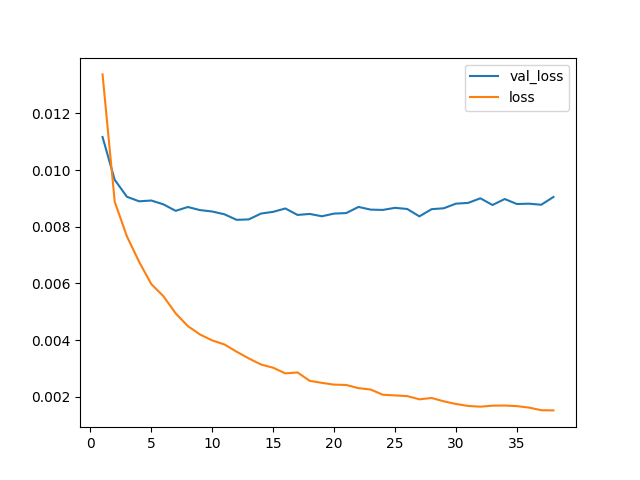
\includegraphics[width=.8\linewidth]{figuras/ape-ajustes-hiper-parametros/shared-cnn-with-bn-2000-k-2-m-005.png}
  \caption{Rede convolucional com parâmetros $F = 2000$, $K = 2$ e $m = 0,05$, normalização em lote e parâmetros compartilhados.}
  \label{fig:shared-cnn-2000-k-2-m-005-normalizacao-em-lote}
\end{subfigure}
\begin{subfigure}{.5\textwidth}
  \centering
  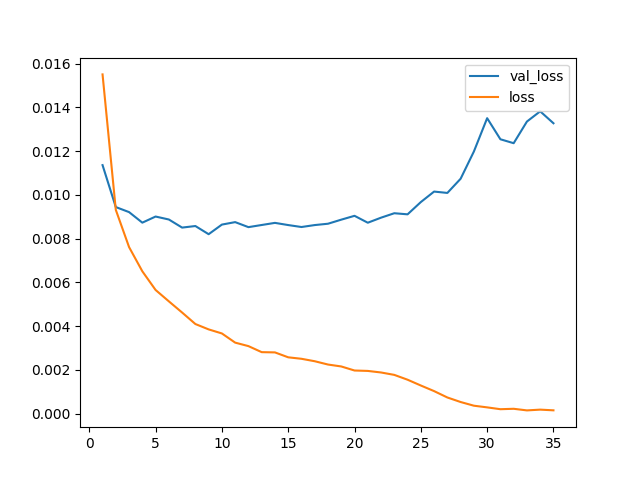
\includegraphics[width=.8\linewidth]{figuras/ape-ajustes-hiper-parametros/cnn-with-bn-4000-k-2-m-005.png}
  \caption{Rede convolucional com parâmetros $F = 4000$, $K = 2$ e $m = 0,05$ e normalização em lote.}
  \label{fig:cnn-4000-k-2-m-005-normalizacao-em-lote-v2}
\end{subfigure}
\begin{subfigure}{.5\textwidth}
  \centering
  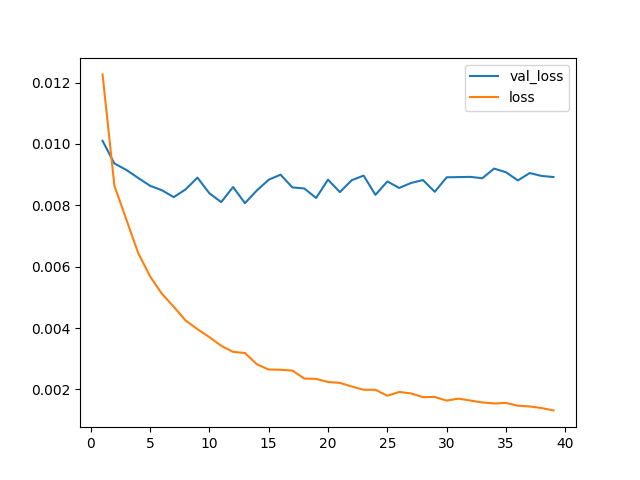
\includegraphics[width=.8\linewidth]{figuras/ape-ajustes-hiper-parametros/shared-cnn-with-bn-4000-k-2-m-005.png}
  \caption{Rede convolucional com parâmetros $F = 4000$, $K = 2$ e $m = 0,05$, normalização em lote e parâmetros compartilhados.}
  \label{fig:shared-cnn-4000-k-2-m-005-normalizacao-em-lote}
\end{subfigure}

\caption{Gráfico do treinamento da rede convolucional na recuperação de trecho de código-fonte. Este gráfico apresenta um comparativo do erro no conjunto de validação em comparação com o erro no conjunto de treinamento. Mais detalhes sobre o treinamento, ver a Seção~\ref{sec:treinamento}. O parâmetro F indica a quantidade de filtros convolucionais, o parâmetro K indica o tamanho da janela do filtro convolucional e o parâmetro \emph{m} é a margem utilizada na função de perda \textit{hinge}. Nas figuras de \emph{a} a \emph{f}, o eixo \emph{y} indica o valor de erro da função de perda \textit{hinge}, já o eixo \emph{x} indica as épocas de treinamento. A legenda \emph{val\_loss} das figuras de \emph{a} a \emph{g} indica o erro na amostra de validação e a legenda \emph{loss} indica o valor do erro na amostra de treinamento. Nas figuras do lado esquerdo: \emph{a}, \emph{c} e \emph{e} apresentam o comportamento das redes convolucionais que aprenderam as representações de forma independente, sem o compartilhamento de parâmetros. As figuras do lado direito: \emph{b}, \emph{d} e \emph{f} apresentam o comportamento das redes convolucionais que compartilharam os parâmetros durante a aprendizagem de representação das questões e trechos de código-fonte. }
\label{fig:treinamento-shared-cnn}
\end{figure}

\begin{table}[H]
\centering
\begin{tabular}{ p{1cm} p{4cm} P{4cm} P{4cm} }
 \hline
    & & \multicolumn{2}{c}{\textbf{Resultados MRR}}\\
 \hline
 & \textbf{Modelos} & \textbf{Independente} & \textbf{Compartilhado}\\
 \hline
 
 C1 & CNN / F = 1000 &  $0.682$ & \cellcolor{Gray!35} $0,690$\\
 
 C2 & CNN / F = 2000 &  $0.689$ & \cellcolor{Gray!35}$0,700$\\
 
 C3 & CNN / F = 4000 &  $0.688$ & \cellcolor{Gray!35}$0,701$\\
 
\hline
\end{tabular}
\caption{Resultado da avaliação dos modelos CNN na amostra EVAL. MRR refere-se a média do resultado do Mean Reciprocal Rank (equação~\ref{eq:mrr}). F indica a quantidade de filtros convolucionais utilizados durante o treinamento das redes convolucionais. \emph{NL} é o acrônimo de Normalização em Lote. As células destacadas indicam qual o modelo obteve o melhor desempenho durante a avaliação. Os hiper-parâmetros utilizados foram: $K = 2$ e  $m = 0,05$. A coluna \emph{Independente} indicam os modelos que não compartilharam os parâmetros na aprendizagem de representação das questões e trechos de código-fonte. A coluna \emph{Compartilhado} apontam para os modelos que compartilharam os parâmetros durante a aprendizagem de representação dos pares.}
\label{table:tabela-shared-cnn}
\end{table}



\section{Ajuste da margem - Função de perda hinge}

Além dos hiper-parâmetros das redes convolucionais, a função de perda \textit{hinge} conforme descrito na Seção~\ref{sec:funcao-objetivo}, exige um parâmetro \emph{margem}. Este parâmetro define a magnitude da diferença da distância de similaridade entre os trechos de códigos anotados como corretos e os trechos que não são respostas com relação às questões. Os pesquisadores \cite{feng-2015} recomendaram uma margem de $0,009$, enquanto \cite{tan-lstm-qa} utilizaram uma margem de $0,2$. Em nosso caso, fizemos alguns experimentos com os valores $0,009$, $0,05$, $0,1$ e $0,2$. 


\begin{table}[H]
\centering
\begin{tabular}{ p{1cm} p{4cm} P{2.2cm} P{2.2cm} P{2.2cm} P{2.2cm} }
 \hline
    & & \multicolumn{4}{c}{\textbf{Resultados MRR}}\\
 \hline
 & \textbf{Modelos} & \textbf{$m = 0,009$} & \textbf{$m = 0,05$} & \textbf{$m = 0,1$}& \textbf{$m = 0,2$}\\
 \hline
 A1 & Embedding & $0.600$& $0.632$& \cellcolor{Gray!35} $0.637$& $0.635$\\
 
 \hline
 \
 B1 & Unif & $0.647 $ & $0.652$& $0.660$& \cellcolor{Gray!35} $0.674$\\
 
 \hline
 
 C1 & CNN / F = 1000 & $0.654 $ & $0.669$& \cellcolor{Gray!35} $0.676$& $0.637$\\
 
 C2 & CNN / F = 2000 & $0.675 $ & \cellcolor{Gray!35} $0.673$& $0.661$& $0.647$\\
 
 C3 & CNN / F = 4000 & $0.664$ & \cellcolor{Gray!35} $0.687$& $0.672$& $0.651$\\
 
\hline
\end{tabular}
\caption{Resultado da avaliação dos modelos CNN, \Gls{unif} e Embedding na amostra EVAL. MRR refere-se a média do resultado do Mean Reciprocal Rank (equação~\ref{eq:mrr}). O hiper-parâmetro \emph{m} indica a margem utilizada na função de perda \textit{hinge}. F indica a quantidade de filtros convolucionais utilizados durante o treinamento das redes convolucionais. As células destacadas indicam a margem na qual o modelo obteve o melhor desempenho durante a avaliação.}
\label{table:alteracao-margem}
\end{table}



Notamos que não há um consenso sobre o valor da margem, conforme a Tabela~\ref{table:alteracao-margem}, pois cada arquitetura obteve um desempenho diferente para um valor diferente de margem. As redes convolucionais obtiveram o melhor desempenho para uma margem de valor $0,05$, exceto quando a quantidade de filtros convolucionais utilizadas é $1000$. Já a arquitetura Unif proposta por \cite{cambronero-deep-learning-code-search:2019} obteve o melhor desempenho para o valor $0,2$, enquanto a arquitetura \textit{Embedding} obteve com o valor $0,1$. Optamos por fixar estes valores específicos para cada arquitetura, definindo a margem em $0,5$ para a CNN, enquanto para Unif e \textit{Embedding} fixamos em $0,2$ e $0,1$, respectivamente. E conforme descrito na Tabela~\ref{table:alteracao-margem}, escolhemos o valor da margem baseado no valor mais alto da métrica MRR, que foi obtida através da avaliação do melhor modelo na amostra EVAL. Ver a Seção~\ref{sec:avaliacao} para mais detalhes sobre o procedimento de avaliação. 



\section{Escolha do melhor modelo}

Para treinamento e avaliação, utilizamos o procedimento descrito por \cite{iyer-etal-2016-summarizing}. No caso do treinamento, ao final de cada época, avaliamos o modelo em uma amostra contendo pares de questões e trechos de código-fonte anotados manualmente. O modelo que obtiver a maior média MRR nesta amostra é utilizado na avaliação final. Este procedimento está descrito com mais detalhes na Seção~\ref{sec:treinamento}. Tanto \cite{iyer-etal-2016-summarizing} quanto \cite{yao-2018} verificaram que este procedimento levaram à escolha do melhor modelo com relação a métrica MRR. Para verificar esta afirmação, adotamos este procedimento de \cite{iyer-etal-2016-summarizing} e comparamos com um outro procedimento comumente utilizado, onde o modelo escolhido é o modelo que obtiver o menor valor do erro na amostra de validação. Conforme os resultados da Tabela~\ref{table:escolha-melhor-modelo}, não houve uma diferença significativa no desempenho entre as formas de escolha do modelo. No nosso caso, optamos por manter o mesmo procedimento adotado por \cite{iyer-etal-2016-summarizing} e \cite{yao-2018}.


\begin{table}[H]
\centering
\begin{tabular}{ p{1cm} p{4cm} P{4cm} P{4cm} }
 \hline
    & & \multicolumn{2}{c}{\textbf{Resultados MRR}}\\
 \hline
 & \textbf{Modelos} & \textbf{MRR} & \textbf{Erro de validação}\\
 \hline
 A1 & Embedding & $0.637$& $0.637$\\
 
 \hline
 \
 B1 & Unif & $0.674 $ & $0.673$\\
 
 \hline
 
 C1 & CNN / F = 1000 & $0.690 $ & $0.684$\\
 
 C2 & CNN / F = 2000 & $0.700 $ & $0.694$\\
 
 C3 & CNN / F = 4000 & $0.701$ & $0.688$\\
 
\hline
\end{tabular}
\caption{Resultado da avaliação dos modelos CNN, \Gls{unif} e Embedding na amostra EVAL. MRR refere-se a média do resultado do Mean Reciprocal Rank (equação~\ref{eq:mrr}). Utilizamos normalização em lote e compartilhamento de parâmetros nas redes convolucionais. Os hiper-parâmetros utilizados nas redes convolucionais foram: $K = 2$ e $m = 0,05$. Já a rede \emph{Embedding} utilizou o parâmetro $m = 0,1$. E a arquitetura \emph{Unif} utilizou o parâmetro $m = 0,2$. F indica a quantidade de filtros convolucionais utilizados durante o treinamento das redes convolucionais. A coluna \emph{Erro de validação} indica os resultados dos modelos que foram escolhidos com base no erro na amostra de validação. A coluna \emph{MRR} indicam os resultados dos modelos que foram escolhidos com base na métrica MRR.}
\label{table:escolha-melhor-modelo}
\end{table}